\begin{frame}{\IS}
    \begin{minipage}{0.5\textwidth}
        \begin{alertblock}{\IS}
            \textbf{Input:}
            \begin{itemize}
                \item<2-> A graph $G = (V, E)$,
                \item<3-> An integer $k \in \N$.
            \end{itemize}

            \textbf{Output:}
            
            \onslide<4->{Yes if there is ${\color{red}X} \subseteq V$ s.t}
            \begin{itemize}
                \item<5-> $|X| \geq k$,
                \item<6-> $G[X]$ has no edge.
            \end{itemize}
        \end{alertblock}
    \end{minipage}
    \begin{minipage}{0.45\textwidth}
        \centering
        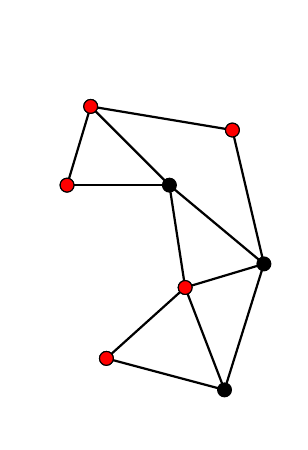
\begin{tikzpicture}
    \tikzstyle{vertex} = [draw=black,fill=black,circle,inner sep=0pt,minimum size=5pt];
    \tikzstyle{chosen} = [draw=black,fill=red,circle,inner sep=0pt,minimum size=5pt];
    \tikzstyle{edge} = [draw=black,thick];

    % This is an invisible rectangle which draw the picture to avoid nodes to move when appear/disappear.
    \path (0, 0) -- (3.2, 0) -- (3.2, 5) -- (0, 5);

    \coordinate (A) at (.5, 3);
    \coordinate (B) at (.8, 4);
    \coordinate (C) at (1, .8);
    \coordinate (D) at (1.8, 3);
    \coordinate (E) at (2, 1.7);
    \coordinate (F) at (2.5, 0.4);
    \coordinate (G) at (2.6, 3.7);
    \coordinate (H) at (3, 2);

    \node<2-5,7-> [style=vertex] at (A) {};
    \node<2-5,7-> [style=vertex] at (B) {};
    \node<2-5,7-> [style=vertex] at (C) {};
    \node<2-5,7-> [style=vertex] at (D) {};
    \node<2-5,7-> [style=vertex] at (E) {};
    \node<2-5,7-> [style=vertex] at (F) {};
    \node<2-5,7-> [style=vertex] at (G) {};
    \node<2-5,7-> [style=vertex] at (H) {};

    \draw<2-5,7-> [style=edge] (A) -- (B);
    \draw<2-5,7-> [style=edge] (A) -- (D);
    \draw<2-5,7-> [style=edge] (B) -- (D);
    \draw<2-5,7-> [style=edge] (B) -- (G);
    \draw<2-5,7-> [style=edge] (C) -- (E);
    \draw<2-5,7-> [style=edge] (C) -- (F);
    \draw<2-5,7-> [style=edge] (D) -- (E);
    \draw<2-5,7-> [style=edge] (D) -- (H);
    \draw<2-5,7-> [style=edge] (E) -- (F);
    \draw<2-5,7-> [style=edge] (E) -- (H);
    \draw<2-5,7-> [style=edge] (F) -- (H);
    \draw<2-5,7-> [style=edge] (G) -- (H);

    \node<4-7> [style=chosen] at (B) {};
    \node<4-7> [style=chosen] at (E) {};

    \node<8> [style=chosen] at (A) {};
    \node<8> [style=chosen] at (C) {};
    \node<8> [style=chosen] at (G) {};
\end{tikzpicture}

        \onslide<3->{$k = 2$}
    \end{minipage}
\end{frame}

\begin{frame}{Parameterized complexity}
    \begin{center}
        $\IS$ is \NP-complete.
    \end{center}

    \vspace*{1cm}

    \begin{itemize}
        \item<2-> Algorithm in \only<2-4>{$\O(\varphi^n\cdot n^{\O(1)})$}\only<5->{${\color<5>{red}\O^\star}(\varphi^n)$} \qquad $\varphi \approx 1.618$
        \item<3-> Algorithm in \only<2-4>{$\O(2^k\cdot n^{\O(1)})$}\only<5->{${\color<5>{red}\O^\star}(2^k)$}
    \end{itemize}

    \vspace*{1cm}

    \onslide<4->{Interesting if $k$ is small.}

    \onslide<6->{But what about other \textbf{parameters}?}
\end{frame}

\begin{frame}{Hierarchy of parameters}
    \begin{minipage}{0.5\textwidth}
        \centering
        \begin{tikzpicture}
    \tikzstyle{vertex} = [draw=black,fill=black,circle,inner sep=0pt,minimum size=3pt];
    \tikzstyle{possible} = [fill=green,circle,inner sep=0pt,minimum size=10pt];
    \tikzstyle{impossible} = [fill=red,circle,inner sep=0pt,minimum size=10pt];
    \tikzstyle{new} = [fill=lime,circle,inner sep=0pt,minimum size=10pt];
    \tikzstyle{result} = [draw=black,circle,dashed,thick,inner sep=0pt,minimum size=20pt];
    \tikzstyle{edge} = [draw=black,thick];
    \tikzstyle{possibleedge} = [draw=green,line width=5pt];
    \tikzstyle{impossibleedge} = [draw=red,line width=5pt];
    \tikzstyle{newedge} = [draw=lime,line width=5pt];

    % This is an invisible rectangle which draw the picture to avoid nodes to move when appear/disappear.
    \path (0, 0) -- (3.2, 0) -- (3.2, 5) -- (0, 5);

    \coordinate (A) at (2, 4.6);
    \coordinate (B) at (2, 3.8);
    \coordinate (C) at (2, 3);
    \coordinate (D) at (1, 1.7);
    \coordinate (E) at (1, .7);
    \coordinate (F) at (0, 0);
    \coordinate (G) at (3.5, 3);
    \coordinate (H) at (3, 2.5);
    \coordinate (I) at (3, 1.5);
    \coordinate (J) at (3, .5);
    \coordinate (K) at (2, 0);

    \node<3-> [style=possible] at (A) {};
    \node<4-> [style=possible] at (B) {};
    \node<7-> [style=possible] at (G) {};

    \draw<4-> [style=possibleedge] (A) -- (B);

    \node<6-> [style=impossible] at (I) {};
    \node<5-> [style=impossible] at (J) {};
    \node<5-> [style=impossible] at (K) {};

    \draw<6-> [style=impossibleedge] (I) -- (J);
    \draw<5-> [style=impossibleedge] (J) -- (K);

    \node<8-> [style=new] at (C) {};
    \node<8-> [style=new] at (D) {};
    \node<8-> [style=new] at (E) {};
    \node<8-> [style=new] at (F) {};
    \node<9-> [style=new] at (H) {};

    \draw<8-> [style=newedge] (B) -- (C);
    \draw<8-> [style=newedge] (C) -- (D);
    \draw<9-> [style=newedge] (C) -- (H);
    \draw<8-> [style=newedge] (D) -- (E);
    \draw<8-> [style=newedge] (E) -- (F);
    \draw<9-> [style=newedge] (G) -- (H);

    \node<8-> [style=result] at (F) {};
    \node<9-> [style=result] at (H) {};
    \node<10-> [style=result] at (I) {};

    \node [style=vertex,label={[label distance=1pt]180:$n$}]        at (A) {};
    \node [style=vertex,label={[label distance=1pt]180:\vc}]        at (B) {};
    \node [style=vertex,label={[label distance=1pt]180:$\shub[2]$}] at (C) {};
    \node [style=vertex,label={[label distance=1pt]170:\lfvs}]      at (D) {};
    \node [style=vertex,label={[label distance=1pt]170:\fvs}]       at (E) {};
    \node [style=vertex,label={[label distance=1pt]270:\oct}]       at (F) {};
    \node [style=vertex,label={[label distance=1pt]90:$\sdhub$}]   at (G) {};
    \node [style=vertex,label={[label distance=1pt]0:$\shub$}]    at (H) {};
    \node [style=vertex,label={[label distance=1pt]0:\td}]        at (I) {};
    \node [style=vertex,label={[label distance=1pt]0:\pw}]        at (J) {};
    \node [style=vertex,label={[label distance=1pt]270:\tw}]        at (K) {};

    \draw [style=edge] (A) -- (B);
    \draw [style=edge] (B) -- (C);
    \draw [style=edge] (C) -- (D);
    \draw [style=edge] (C) -- (H);
    \draw [style=edge] (D) -- (E);
    \draw [style=edge] (D) -- (J);
    \draw [style=edge] (E) -- (F);
    \draw [style=edge] (E) -- (K);
    \draw [style=edge] (G) -- (H);
    \draw [style=edge] (H) -- (I);
    \draw [style=edge] (I) -- (J);
    \draw [style=edge] (J) -- (K);
\end{tikzpicture}
    \end{minipage}
    \begin{minipage}{0.47\textwidth}
        \begin{itemize}
            \item<3-> $\O^\star(\varphi^n)$
            \item<4-> $\O^\star(1.4656^\vc)$
            \item<5-> No $\O^\star((2 - \varepsilon)^\pw)$ (2011)
            \item<6-> No $\O^\star((2 - \varepsilon)^\td)$ (2024)
            \item<7-> $\exists. \varepsilon\ \O^\star((2 - \varepsilon)^{\sdhub})$ (2024)
        \end{itemize}

        \medskip

        \begin{itemize}
            \item<8-> \color{red} $\O^\star(1.53^\oct)$
            \item<9-> \color{red} $\exists. \varepsilon\ \O^\star((2 - \varepsilon)^{\shub})$
            \item<10-> \color{red} No $\O^\star((2 - \varepsilon)^\td)$
        \end{itemize}
    \end{minipage}

    \medskip

    \pause 

    Given a parameter $p$, does it exist an algorithm for \IS\ in time $\O^\star((2-\varepsilon)^p)$ for any $\varepsilon > 0$?
\end{frame}